\documentclass[11pt]{article}
\usepackage[margin=1in]{geometry}
\usepackage[T1]{fontenc}
\usepackage[utf8]{inputenc}
\usepackage{lmodern}
\usepackage{microtype}
\usepackage{amsmath,amssymb}
\usepackage{graphicx}
\usepackage{booktabs}
\usepackage{tabularx}
\usepackage{array}
\usepackage[font=small,labelfont=bf]{caption}
\usepackage[hidelinks]{hyperref}
\graphicspath{{figures/}}
\newcolumntype{Y}{>{\raggedright\arraybackslash}X}
\setlength{\parskip}{0.4em}
\setlength{\parindent}{0pt}
\renewcommand{\topfraction}{0.9}
\renewcommand{\bottomfraction}{0.8}
\renewcommand{\textfraction}{0.07}
\renewcommand{\floatpagefraction}{0.8}
\setcounter{topnumber}{3}

\title{What Does POYO Learn About Neurons?}
\author{\textbf{Shrivatsa Deshmukh}\\
University of Minnesota -- Twin Cities\\
\texttt{deshm080@umn.edu}}
\date{}

\begin{document}
\maketitle

\begin{abstract}
POYO is a transformer that decodes behaviour from many neurons by turning every spike into a token: a learned vector for the neuron that fired (its \emph{unit embedding}) and the spike's exact time. We test what the public POYO-MP model has learned, using the 99 sessions of monkey motor cortex it was trained on and no retraining. Two analyses test the unit embeddings. (i) Giving each neuron the embedding learned for the same electrode on another day keeps 71\% of decoding accuracy, whereas random electrodes keep none; pooling three nearby days and matching neurons by firing rate, without behaviour labels, raises this to 91\%. The transfer fades over months, and because the sessions were part of training, this cross-day test is a simulated one. (ii) The embeddings describe each neuron: a linear readout recovers its preferred movement direction (median error 21.5$^\circ$) and firing rate, which the model was never given. They also fit a small shared code: 256 shared codes keep 86\% of accuracy and 16 shared axes keep 96\%; across monkeys, the axes carry over but the codes do not. Two analyses test the network. (iii) A neuron that stops recording should be left out rather than shown as silent, which roughly halves the damage when most neurons are lost. (iv) Fine spike timing is barely used: moving spikes by up to 20 ms costs less than 0.001 R$^{2}$.
\end{abstract}

\section{Introduction}

Brain-computer interfaces decode movement from neurons recorded by implanted electrodes, but the recorded neurons change from day to day, so decoders usually need to be recalibrated. POYO~\cite{ref1} offers a different route: a single model trained on many sessions at once. Every spike becomes one token, so a session with any number of neurons can be read. Every recorded neuron (a \emph{unit}) gets its own learned vector, its \emph{unit embedding}, and every session gets a \emph{session embedding}, so the model can tell neurons apart. The tokens are compressed by a Perceiver IO backbone~\cite{ref2}. For a new session, POYO learns new embeddings from labelled data (``unit identification'').

The POYO paper motivates this design with claims about what the model learns. The unit embeddings are said to encode ``something about the 'speaker's' identity and role in neural computation''; training on many sessions is said to give a representation that transfers to new recordings; and spike tokens are said to preserve ``the neural code's finest temporal structure''. The paper tests these claims mainly through decoding accuracy after training. Its closest test of the embeddings shows that unit identification on a session already seen in training recovers embeddings close to the original ones~\cite{ref1}; what the embeddings encode is left for future work. Whether they carry over to other days has not been tested, and neither has whether a trained model \emph{uses} the fine timing that its tokens preserve.

In this work, we test what POYO's unit embeddings encode and how its network uses its tokens. We study the public POYO-MP model, trained to decode hand movements from monkey motor cortex~\cite{ref3}, and train no models. Instead, we probe the frozen model in four ways (Figure 1): the first two test its unit embeddings, and the last two test how the network uses its tokens.

\begin{itemize}
\item \textbf{Another day's embeddings decode a session.} Same-electrode embeddings from a nearby day decode a session with no learning, and pooling days and matching neurons by firing rate, without behaviour labels, recovers most of the accuracy. The transfer fades over months, and POYO fails gracefully where a linear decoder does not.
\item \textbf{The embeddings describe each neuron.} They encode each neuron's preferred movement direction and firing rate, and units recorded on the same electrode on different days look alike, consistent with the transfer. They also fit a small shared code: a few hundred shared codes, or 16 shared axes, keep most of the accuracy, and the axes carry over between monkeys.
\item \textbf{When neurons go missing, absent beats silent.} A neuron that stops recording should be left out of the input rather than shown as silent.
\item \textbf{Fine spike timing is barely used.} Moving spikes by tens of milliseconds costs almost nothing, and a simple linear decoder breaks down at the same coarse bin sizes as POYO.
\end{itemize}

All sessions we use were part of POYO-MP's training, so each ``new day'' is simulated: the model has seen that day's data before, and only its embeddings are borrowed from another day.

\section{Approach}

\begin{figure}[!tbp]
\centering
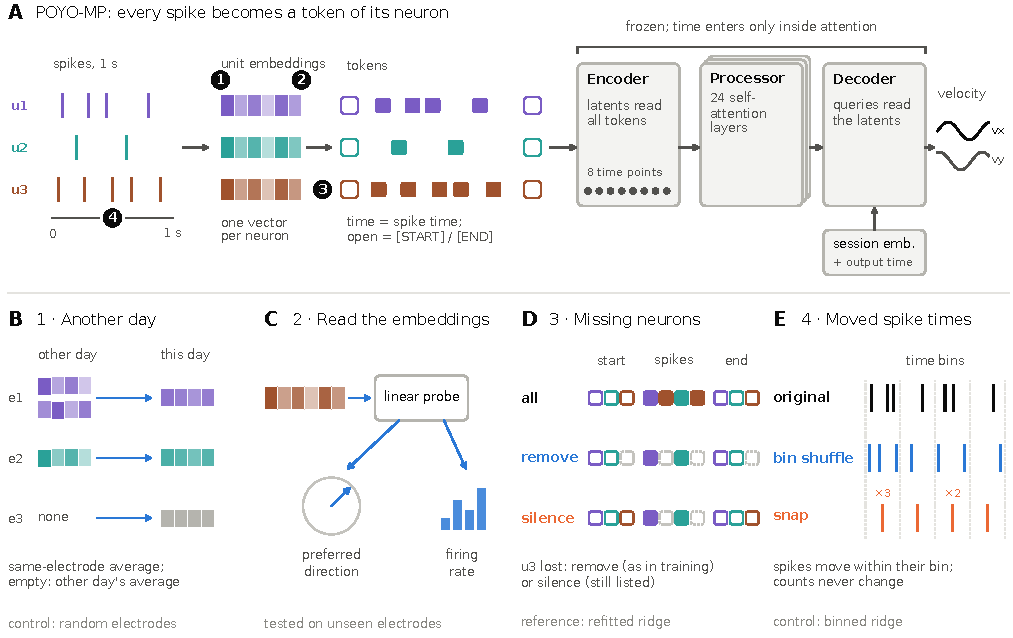
\includegraphics[width=\linewidth]{fig1_overview}
\caption{\textbf{POYO-MP and our four analyses.} (A) Each spike in a 1 s window becomes a token whose
vector is the learned embedding of the unit that fired (one colour per unit) and whose time is the
spike time; each unit also adds a [START] and an [END] token (open squares), so that silent units
are still visible. Time enters the model only inside attention. Latent tokens read all tokens, are
processed by 24 layers, and are read out by queries built from the session embedding. The model is
never retrained. Numbered markers show where each analysis acts; the numbers match the panels below
and Figure 2. (B) Each unit receives the average embedding of the other day's units on the same
electrode, or the other day's average if that electrode recorded nothing. (C) A linear probe
predicts each neuron's preferred direction and firing rate from its embedding. (D) A lost unit is
either removed (all its tokens deleted, as in training) or silenced (only its spike tokens deleted).
(E) Spikes are moved to the centre of their time bin (snap) or to a random time within it (bin
shuffle). Blue and orange mark the two conditions compared in Figure 2.}
\end{figure}

\subsection{POYO-MP}

\textbf{Tokens.} POYO-MP reads 1 s windows of spikes. Each spike becomes a token whose vector is the unit embedding of the neuron that fired (128 numbers) and whose time is the spike time. Because spikes only record activity, each unit also contributes a [START] and an [END] token at the edges of the window, called \emph{delimiter tokens}. They tell the model which units are being recorded, even when a unit does not fire.

\textbf{Model.} A small set of latent tokens, spread over the window every 125 ms, reads all the tokens at once and passes the result through 24 attention layers. Queries then read the latents at each time point to predict the hand's velocity. Every query of a session is the same vector, its session embedding. Time is never stored in the vectors; it enters only through rotary encoding~\cite{ref4} inside each attention layer, so the model sees only time differences between tokens (Appendix A.1).

\textbf{Training.} POYO-MP was trained with \emph{unit dropout}: in each training window, a random number of units was left out, together with their delimiter tokens. This matters for Section 3.3.

\subsection{Data and evaluation}

We use the public POYO-MP checkpoint and the \texttt{torch\_brain} library~\cite{ref5} without changes. The data are the 99 public sessions the model was trained on~\cite{ref3}: three monkeys making reaching movements in two tasks, center-out (CO, 78 sessions) and random-target (RT, 21 sessions), with 9,725 units recorded from motor (M1) and premotor (PMd) cortex by chronic electrode arrays. We decode hand velocity on each session's held-out test trials and score it with R$^{2}$, the share of the velocity's variance that the decoder explains. The unmodified model reaches R$^{2}$ 0.949 on CO and 0.869 on RT, matching the paper (Appendix A.2). Every analysis below is scored against this baseline.

\subsection{Analyses}

\textbf{Reusing embeddings on another day.} For each session, we replace its unit embeddings, in memory and without any training, with those learned for the nearest other recording day of the same monkey and task. Because the arrays stay implanted, we match units by electrode: each unit receives the average embedding of the other day's units on the same electrode, or the other day's overall average if that electrode recorded nothing. As controls, we pair electrodes at random, or give every unit the same average vector. We then improve the matching, still without learning: we pool the three nearest days, and on each electrode we pick the other-day unit whose firing (rate and regularity) is most similar, which uses only spike times. We also vary the time between the two days, swap the session embedding, and compare with a linear decoder (ridge regression on spike counts) trained on another day, or averaged over the same three days, and applied unchanged.

\textbf{Reading the embeddings.} From the recordings alone, we measure each neuron's firing rate and how it is tuned to movement: its preferred direction, and how strongly it is tuned. We then fit a linear readout, called a \emph{probe}, that predicts each property from the neuron's embedding, and test it on neurons it has not seen. To make the test strict, all neurons recorded on the same electrode, on any day, are held out together. We compare the probe with a baseline that only knows which session a neuron came from. We also ask how compact the embeddings are: we replace every embedding of a session with its nearest code in a \emph{codebook} learned from other sessions or from other monkeys, or keep only its position on a few principal axes, and measure how much decoding survives.

\textbf{Losing neurons.} We take away 10\% to 75\% of each session's units in two ways. In \emph{remove}, a unit's spike tokens and its delimiter tokens are deleted, as in unit dropout during training, so the model sees a smaller population. In \emph{silence}, only its spike tokens are deleted, so the model still sees the unit listed but never firing. Both use the same units. As a reference, we retrain the linear decoder from scratch on the remaining units.

\textbf{Moving spike times.} Before the spikes reach the model, we move each one to a new time while keeping every neuron's spike count. We cut time into bins of a given size, from 1 to 500 ms, and move each spike either to the centre of its bin (\emph{snap}) or to a random time within its bin (\emph{bin shuffle}). If the model relies on timing finer than the bin size, accuracy should drop. A drop could also mean that the movement itself changes too fast for that bin size, so we also train the linear decoder on spike counts in bins of each size and see where it breaks down.

\section{Results}

Table 1 summarises our four questions and their answers, and Figure 2 shows one result for each.

\begin{table}[!tbp]
\centering
\small
\caption{\textbf{Our four questions and their answers.} Full results in Appendices B and C.}
\begin{tabularx}{\linewidth}{lYYY}
\toprule
 & question & answer & key control \\
\midrule
1 & Can another day's embeddings decode a session? & Mostly: 71\% of R$^{2}$ kept with same-electrode embeddings from the nearest day; 91\% with three days and firing-rate matching & Random electrodes: 0\%; a linear decoder moved across days: 68\% (one day), 75\% (three days) \\
2 & What do the unit embeddings encode? & Each neuron's properties: preferred direction to 21.5$^\circ$, firing rate R$^{2}$ 0.56; 256 shared codes keep 86\% of R$^{2}$, 16 shared axes 96\% & Knowing only the session: 73$^\circ$, R$^{2}$ 0.15; random codes: 0\% \\
3 & Is a missing neuron better absent or silent? & Absent: with 75\% of units lost, $\Delta$R$^{2}$ $-$0.31 (removed) vs $-$0.57 (silenced) & A linear decoder retrained on the remaining units loses more of its accuracy \\
4 & Does the model use fine spike timing? & Barely: moving spikes by up to 20 ms costs < 0.001 R$^{2}$, by up to 50 ms < 0.005 R$^{2}$ & A linear decoder trained at each bin size breaks down at the same bin sizes (100--333 ms) \\
\bottomrule
\end{tabularx}
\end{table}

\begin{figure}[!tbp]
\centering
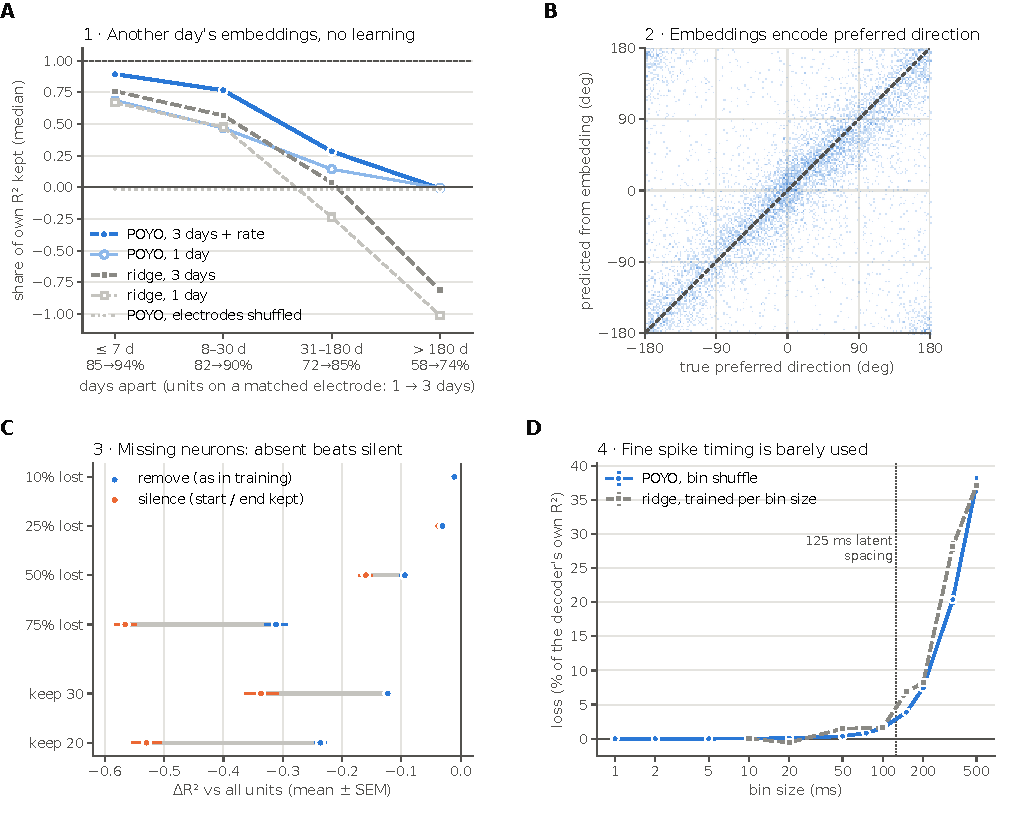
\includegraphics[width=\linewidth]{fig2_results}
\caption{\textbf{Results, one panel per question.} (A) Share of R$^{2}$ kept with another day's embeddings,
against the time between the two days: POYO with three days and firing-rate matching (blue), POYO
with one day's same-electrode embeddings (light blue), a linear decoder moved across days (grey,
dashed; three days averaged, and one day in light grey), and POYO with random electrodes (dotted);
medians across sessions. Below each bin: share of units on a matched electrode with one and with
three days. (B) Each neuron's true preferred direction against the direction predicted from its
embedding, for 8,615 well-tuned neurons not seen by the probe. (C) Loss in R$^{2}$ when units are lost,
by removing them (blue) or silencing them (orange). (D) Loss in accuracy, as a percentage of each
decoder's own R$^{2}$, when spikes are shuffled within bins of a given size: POYO-MP (blue) and a linear
decoder trained at each bin size (grey, dashed); the dotted line marks the 125 ms spacing of POYO's
latent tokens. Means $\pm$ SEM across sessions in C and D.}
\end{figure}

\subsection{Another day's embeddings decode a session}

\textbf{Same-electrode embeddings keep most of the accuracy.} Borrowing the embeddings of the same electrodes from the nearest other day keeps a median 71\% of a session's R$^{2}$, with no learning. Pairing electrodes at random within the same brain area keeps nothing, and so does giving every unit the same average vector. So POYO needs the right identity for each unit, and the electrode provides it.

\textbf{The session embedding barely matters.} Replacing a session's embedding with that of another monkey's session costs almost nothing in most sessions. What makes a session decodable lives mainly in its unit embeddings.

\textbf{Pooling days and matching firing.} Simple matching has two weaknesses. First, in 11\% of units the electrode recorded nothing on the other day, so the unit only gets an average vector. Borrowing from the three nearest days instead of one leaves just 5\% of units without a match, and raises the share kept from 71\% to 84\%. Second, when an electrode recorded several units, simple matching gives each unit their average. Giving each unit instead the embedding of the one unit on its electrode with the most similar firing (rate and regularity) also raises the share kept to 84\%. With both fixes, 91\% is kept, and the gain over simple matching holds in 86\% of sessions. Both fixes use only the recorded spikes, not the movements, so they need no labelled data. Firing similarity helps only within an electrode: matching units by firing alone, ignoring electrodes, keeps just 3\%.

\textbf{Transfer fades with time and fails gracefully.} With the improved matching, the share kept falls from 89\% for days less than a week apart to 28\% at one to six months, and to 0\% beyond six months (Figure 2A). A linear decoder moved across days keeps 68\%, or 75\% averaged over the same three days, less than POYO. On distant days it becomes much worse than predicting nothing, whereas POYO falls back to R$^{2}$ $\approx$ 0.

\subsection{The embeddings describe each neuron}

\textbf{The embeddings encode the neuron's properties.} A linear probe recovers a neuron's firing rate (R$^{2}$ 0.56) and its preferred movement direction (median error 21.5$^\circ$) from its embedding alone, for neurons on electrodes it has never seen (Figure 2B). A baseline that knows only the session does far worse (R$^{2}$ 0.15 and 73$^\circ$), and shuffled labels give nothing.

\textbf{They describe individual neurons, not sessions.} The probe works just as well when comparing neurons within a single session, and the session explains only 2.4\% of the variation between embeddings. The model was never told any of these properties.

\textbf{The same electrode gives similar embeddings across days.} Units recorded on the same electrode on different days have more similar embeddings than units on different electrodes. The similarity fades from about 0.25--0.29 within a week to about 0.01 after two to three years, which mirrors how the transfer in Section 3.1 fades. This is what we expect if an electrode partly records the same neurons over time, though we cannot prove that the neurons are the same.

\textbf{A small shared code describes the embeddings.} Replacing every embedding of a session with the nearest of 256 codes, learned from other sessions, keeps 86\% of its R$^{2}$; giving each neuron a random code, or one code per brain area, keeps nothing. Keeping only each neuron's position on 16 principal axes keeps 96\%, and 32 axes keep all of it. So no small set of neuron types suffices: accuracy grows steadily with the number of codes instead of saturating at a few, and most of the identity lies in about 16--32 shared directions. Across monkeys, the 16 axes learned from the other monkeys still keep 88\%, but codes learned from them keep only 9\%, because each monkey's neurons occupy their own region of the shared space (Appendix B.3, Figure S3).

\subsection{When neurons go missing, absent beats silent}

\textbf{Absent beats silent.} The direction is expected: POYO-MP was trained with unit dropout, so it has seen units disappear, but not many units fall silent at once. What the test measures is how large the difference is and whether it holds beyond training. From 25\% of units lost onward, removing units always hurts less than silencing them (Figure 2C). With 75\% of units lost, R$^{2}$ drops by 0.31 when they are removed and by 0.57 when they are silenced. The gap persists when fewer units are kept than training ever produced. A unit's delimiter tokens carry its identity even when it sends no spikes, so a silenced unit tells the model ``this neuron is here and completely quiet'' rather than ``this neuron is not recorded''. The same question arises on a new day, when an electrode records nothing.

\textbf{POYO is robust without retraining.} Even without any retraining, POYO loses a smaller share of its accuracy than a linear decoder retrained on the remaining units (10.3\% against 18.7\% with half the units lost).

\subsection{Fine spike timing is barely used}

\textbf{Small shifts cost almost nothing.} Moving spikes by up to 20 ms costs less than 0.001 R$^{2}$, and by up to 50 ms less than 0.005 R$^{2}$ (Figure 2D). At 10 ms, the bin size of the binned decoders that POYO was compared with, the loss is at most 0.0006 R$^{2}$.

\textbf{The model breaks down only at coarse bins, and so does a linear decoder.} Accuracy falls clearly only for bins of 100 ms and more. A linear decoder trained on binned counts breaks down at the same bin sizes, even though it is trained at each one. This suggests that the breakdown reflects how fast the movement changes, about 100--200 ms, rather than a property of POYO.

\section{Discussion}

We probed a pretrained spike-token decoder without retraining it, testing its unit embeddings and how its network uses its tokens. The unit embeddings describe each neuron and, matched by electrode and firing rate, can be borrowed from other days, which fits an electrode partly recording the same neurons over time. The network treats a missing neuron very differently from a silent one, because of its delimiter tokens, and barely uses fine spike timing. What POYO's spike tokens provide, in this setting, is a learned identity for each neuron rather than millisecond timing.

\textbf{What the timing result does and does not say.} We ask whether the trained model \emph{uses} fine timing, not whether spike tokens are a good design. Most of the design's strengths, such as reading any number of neurons and giving each one a learned identity, need one token stream per neuron but not exact spike times, and Sections 3.1--3.2 show that these identities are real and useful. The one benefit that needs exact times, fine timing, is the one the model does not appear to use when decoding hand velocity. This does not show that timing is not \emph{needed}: a model trained without it might do as well or worse, and only retraining can tell. The POYO paper's comparisons with binned decoders change the tokens, the architecture and the training scale at once, so they do not settle this either.

\textbf{Implications.} For a new recording day from the same implant, POYO currently learns new embeddings from labelled data (``unit identification'')~\cite{ref1}. Embeddings borrowed from nearby days by electrode and firing rate need no labels and keep 91\% of accuracy, so they could replace this step for days close in time, or give it a starting point. For brain-computer interfaces built like POYO-MP, an electrode that stops working should be left out of the input rather than shown as silent. Because the embeddings lie on about 16 axes shared between monkeys, a new neuron might need only its position on these axes rather than a new 128-number embedding; we leave this to future work. Real failures are often gradual and affect groups of electrodes, so both points need confirming in practice.

\textbf{Limitations.} The most important limitation concerns the cross-day test: every ``new day'' is a session the model was trained on, so the model has seen its data before and only the embeddings come from another day. The only public sessions POYO-MP never saw come from a different monkey, with no electrodes in common with the training data. This analysis therefore shows that the learned identities carry over between days, not that POYO decodes an unseen day, and it does not test whether training on many sessions makes the model better. All results come from one model and one task. Every change is made at test time to a model trained on unchanged data, so a drop in accuracy can reflect unfamiliar inputs as well as lost information. The probes are linear, the same electrode is not the same neuron, and the lost units are chosen at random. Further limitations are in Appendices B and C.

\section*{Code and data availability}

Code, result files, figures and audit scripts are available at [GITHUB LINK]. Every number in this paper can be checked from the released result files without re-running the experiments. The data are the public \texttt{perich\_miller\_population\_2018} dataset~\cite{ref3} (DANDI 000688), and the model is the public POYO-MP checkpoint~\cite{ref1}.

\section*{Acknowledgements}

This work uses the POYO model and checkpoint~\cite{ref1} and the \texttt{torch\_brain} library~\cite{ref5} from the neuro-galaxy project, and the \texttt{perich\_miller\_population\_2018} dataset of Perich, Miller and colleagues~\cite{ref3}, distributed through DANDI. AI tools were used to help with writing this paper and its code; the author reviewed and takes responsibility for all content.

\begin{thebibliography}{9}
\bibitem{ref1} M. Azabou, V. Arora, V. Ganesh, X. Mao, S. Nachimuthu, M. J. Mendelson, B. Richards, M. G. Perich, G. Lajoie, and E. L. Dyer, ``A unified, scalable framework for neural population decoding,'' \emph{Advances in Neural Information Processing Systems}, vol. 36, 2023.

\bibitem{ref2} A. Jaegle, S. Borgeaud, J.-B. Alayrac, C. Doersch, C. Ionescu, D. Ding, S. Koppula, D. Zoran, A. Brock, E. Shelhamer, et al., ``Perceiver IO: A general architecture for structured inputs \& outputs,'' in \emph{International Conference on Learning Representations}, 2022.

\bibitem{ref3} M. G. Perich, J. A. Gallego, and L. E. Miller, ``A neural population mechanism for rapid learning,'' \emph{Neuron}, vol. 100, no. 4, pp. 964--976, 2018.

\bibitem{ref4} J. Su, Y. Lu, S. Pan, A. Murtadha, B. Wen, and Y. Liu, ``RoFormer: Enhanced transformer with rotary position embedding,'' \emph{arXiv preprint arXiv:2104.09864}, 2021.

\bibitem{ref5} neuro-galaxy, ``torch\_brain,'' version 0.2.0, \url{https://github.com/neuro-galaxy/torch_brain}.
\end{thebibliography}

\clearpage
\appendix
\setcounter{figure}{0}
\renewcommand{\thefigure}{S\arabic{figure}}

\setcounter{table}{0}
\renewcommand{\thetable}{A\arabic{table}}
\section{Model, data and evaluation}

\subsection{POYO-MP}

We use the public POYO-MP checkpoint~\cite{ref1} without changes: embedding dimension 128, one encoder cross-attention layer and one decoder cross-attention layer (4 heads each), 24 processor self-attention layers (8 heads), head dimension 64, and 32 learned latents repeated at 8 time points spaced 125 ms apart in each 1 s window. It was trained for 1,000 epochs with \texttt{UnitDropout(\allowbreak{}min\_units=30,\allowbreak{} mode\_units=100,\allowbreak{} max\_units=300,\allowbreak{} peak=4)}: in each training window, a number of units is drawn from a triangular distribution, and only that many units are kept, together with their [START] and [END] tokens.

\textbf{Relative timing.} Time is never added to the token vectors. Rotary position encoding~\cite{ref4} rotates queries and keys by their timestamps inside every attention layer, so that the attention score between a query at time $t_j$ and a key at time $t_i$,

\[a_{ij} = \mathrm{softmax}\big((R(t_j)\,q_j)^\top R(t_i)\,k_i\big),\]

depends only on $t_i - t_j$. The encoder and processor also rotate the values and rotate each output back by the query time, so that every token's contribution carries its relative time. Of each head's 64 dimensions, 32 are rotated (16 frequencies); the other 32 match tokens on content alone.

\subsection{Data and evaluation}

The data are the 99 public sessions of \texttt{perich\_miller\_population\_2018}~\cite{ref3} in POYO-MP's training configuration: monkey C (68 sessions, 7,043 units), M (28 sessions, 2,607 units) and J (3 sessions, 75 units), all sorted single units from M1 and PMd, with cursor velocity at 100 Hz. The 100th session used in~\cite{ref1} is not in the public release. We follow the validation loop of the POYO example code on the test split of each session (20\% of trials): 1 s windows with a 0.5 s step, predictions averaged over overlapping windows, and R$^{2}$ of cursor velocity (x and y averaged) during the reach period (CO) or the random-target period (RT). The library's stitching averages only predictions with identical timestamps, so some points of overlapping windows enter R$^{2}$ twice (about 0.1\% of points on CO, and 10\% on one RT session checked); all conditions share this path. This reproduces the paper's numbers (Table A1).

\begin{table}[!tbp]
\centering
\small
\setlength{\tabcolsep}{4pt}
\caption{\textbf{Baseline decoding of the unmodified POYO-MP checkpoint on the test split.} The paper reports averages over its 100 training sessions.}
\begin{tabular}{lllll}
\toprule
task & sessions & units & \begin{tabular}[b]{@{}l@{}}R$^{2}$ (this work, \\ mean $\pm$ SEM)\end{tabular} & \begin{tabular}[b]{@{}l@{}}R$^{2}$ reported in \\ ~\cite{ref1}\end{tabular} \\
\midrule
CO & 78 & 7,821 & 0.9488 $\pm$ 0.0021 & 0.9512 \\
RT & 21 & 1,904 & 0.8690 $\pm$ 0.0082 & 0.8738 \\
\bottomrule
\end{tabular}
\end{table}

\subsection{Statistics}

All inference is at the session level: means or medians across sessions, session-bootstrap 95\% confidence intervals, paired Wilcoxon signed-rank tests, and Holm correction over the comparisons within each analysis. Random seeds are fixed and recorded with every result.

\setcounter{table}{0}
\renewcommand{\thetable}{B\arabic{table}}
\section{Tests of the unit embeddings}

\subsection{Another day's embeddings}

\textbf{Swap.} For each target session, its rows of the unit-embedding table (and, in one condition, its session embedding) are overwritten in memory and restored afterwards; tokenization, evaluation and stitching are unchanged. Writing a session's own vectors through this path reproduces its baseline R$^{2}$ exactly in all 99 sessions. A unit's embedding enters its spike tokens and its [START]/[END] tokens; the session embedding enters only the decoder queries.

\textbf{Matching.} The donor is the nearest-date session of the same monkey and task (median 1 day apart). Electrode labels come from the NWB electrode table and include the array, so matches never cross brain areas. Because 71\% of units share their electrode with other units, each unit receives the donor's \emph{average} embedding on its electrode, or the donor's overall average if that electrode recorded nothing on the donor day (a median 11\% of units). In the controls, the donor's electrode labels are re-paired at random (3 seeds, across all electrodes or within M1 and PMd), or every unit receives the donor's average.

\textbf{Label-free improvements.} \emph{3 days} pools the units of the three nearest same-task days (two for monkey J). \emph{Electrode + rate} gives each unit, on a matched electrode, the one donor unit with the most similar firing statistics (log firing rate and inter-spike-interval CV on the training split, standardised), and otherwise the most similar donor unit of the same brain area. \emph{Rate only} does the same while ignoring electrodes. None of these uses behaviour.

\textbf{Days apart.} For each session, one same-task donor is drawn in each of four bins of time apart; the 3-day pool of a bin adds the two same-task sessions of that bin nearest in date to the donor.

\textbf{Fixed ridge.} A ridge decoder on spike counts per electrode (100 ms bins, 300 ms of history; Appendix C.2) is fitted on the donor day and applied unchanged to the target day; electrodes absent on the target day are set to their training mean. With three days, the three decoders' predictions are averaged. \emph{Kept} is R$^{2}$ divided by the session's own reference R$^{2}$ (POYO: the unmodified model; ridge: the session's own decoder, median R$^{2}$ 0.62). We report medians, because a failing ridge decoder can reach R$^{2}$ far below 0.

\begin{table}[!tbp]
\centering
\small
\caption{\textbf{Decoding with unit embeddings from another day (99 sessions).} Every improvement beats matched (better in 83--90\% of sessions, Holm p < 1e-4). 3 days + rate beats both 3 days and electrode + rate (Holm p < 1e-4), which do not differ from each other (p = 0.35). POYO with 3 days + rate beats the 3-day ridge (+0.11, 86\% of sessions, Holm p < 1e-5).}
\begin{tabularx}{\linewidth}{Ylll}
\toprule
condition & R$^{2}$ (median) & \begin{tabular}[b]{@{}l@{}}share of own \\ R$^{2}$ kept, \\ median [95\% \\ CI]\end{tabular} & \begin{tabular}[b]{@{}l@{}}sessions with \\ R$^{2}$ > 0\end{tabular} \\
\midrule
own day, units averaged per electrode & 0.88 & 0.94 [0.92, 0.95] & 100\% \\
\textbf{matched} (1 day, same electrode) & \textbf{0.65} & \textbf{0.71 [0.64, 0.74]} & 99\% \\
electrode + rate & 0.79 & 0.84 [0.81, 0.88] & 98\% \\
3 days & 0.78 & 0.84 [0.80, 0.88] & 100\% \\
\textbf{3 days + rate} & \textbf{0.84} & \textbf{0.91 [0.88, 0.92]} & 100\% \\
rate only (no electrodes) & 0.02 & 0.03 [0.01, 0.04] & 64\% \\
electrodes shuffled within area & $-$0.03 & $-$0.03 [$-$0.04, $-$0.02] & 11\% \\
other day's average for every unit & $-$0.01 & $-$0.01 [$-$0.01, $-$0.00] & 7\% \\
fixed ridge, 1 day & 0.41 & 0.68 [0.62, 0.73] & 90\% \\
fixed ridge, 3 days averaged & 0.44 & 0.75 [0.70, 0.79] & 92\% \\
\bottomrule
\end{tabularx}
\end{table}

\begin{table}[!tbp]
\centering
\scriptsize
\setlength{\tabcolsep}{4pt}
\caption{\textbf{Transfer by time between recordings.} Median share of own R$^{2}$ kept; one same-task donor per bin and session. 3 days + rate beats 1 day in 89\%, 88\% and 73\% of sessions in the first three bins (Holm p < 1e-5) and does not differ beyond 180 days (p = 0.74).}
\begin{tabular}{llllllll}
\toprule
days apart & pairs & median days & \begin{tabular}[b]{@{}l@{}}units matched, \\ 1 $\rightarrow$ 3 days\end{tabular} & POYO, 1 day & \begin{tabular}[b]{@{}l@{}}POYO, 3 days + \\ rate\end{tabular} & \begin{tabular}[b]{@{}l@{}}R$^{2}$ > 0 (3 days \\ + rate)\end{tabular} & \begin{tabular}[b]{@{}l@{}}ridge, 1 $\rightarrow$ 3 \\ days\end{tabular} \\
\midrule
$\leq$ 7 & 93 & 2 & 85\% $\rightarrow$ 94\% & 0.69 & \textbf{0.89} & 99\% & 0.67 $\rightarrow$ 0.76 \\
8--30 & 82 & 14 & 82\% $\rightarrow$ 90\% & 0.47 & \textbf{0.77} & 100\% & 0.48 $\rightarrow$ 0.57 \\
31--180 & 85 & 68 & 72\% $\rightarrow$ 85\% & 0.14 & \textbf{0.28} & 88\% & $-$0.24 $\rightarrow$ 0.04 \\
> 180 & 90 & 463 & 58\% $\rightarrow$ 74\% & $-$0.01 & $-$0.01 & 38\% & $-$1.01 $\rightarrow$ $-$0.81 \\
\bottomrule
\end{tabular}
\end{table}

\begin{figure}[!tbp]
\centering
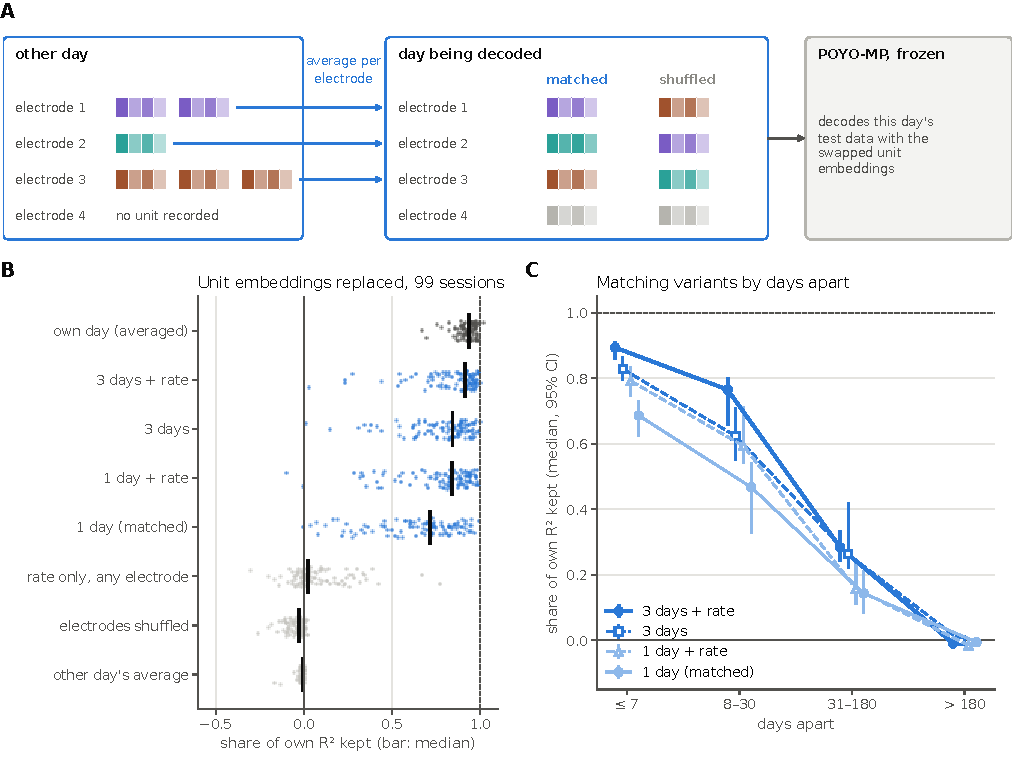
\includegraphics[width=\linewidth]{figS1_transfer}
\caption{\textbf{Another day's embeddings.} (A) Each unit of the day being decoded receives the average
embedding of the other day's units on the same electrode (matched); in the control, the other day's
electrodes are re-paired at random; grey: electrode empty on the other day. (B) Share of each
session's own R$^{2}$ kept when its unit embeddings are replaced (dots: 99 sessions; bar: median). (C)
Median share kept against the time between the two recordings for the four matching variants, with
session-bootstrap 95\% CIs (one same-task donor per bin and session, as in Table B2).}
\end{figure}

\textbf{Further results.} Matched beats the within-area shuffle in every session (+0.64 R$^{2}$ on average, Holm p < 1e-16). Of the 0.33 R$^{2}$ lost by matched, averaging the units of an electrode costs 0.07 even on the same day; the change of day costs the remaining 0.26. Replacing the session embedding with that of another monkey's session costs a median of 0.006 R$^{2}$ (Holm p < 1e-16), except in seven sessions, monkey C's largest (241--353 units), which keep only 40--65\% of their R$^{2}$.

\textbf{Design choices and limitations.} Units on one electrode are different neurons, so we average them rather than pair them arbitrarily; the own-day average measures what this costs. Matching uses firing statistics, not tuning, so that it needs no behaviour labels. Donors have the same task, so that only the day changes. A truly unseen session (for example, monkey T) cannot be decoded this way, because its units have no rows in the embedding table. Donor sessions are shared between the sessions of a monkey, and monkey C contributes 68 of the 99 sessions.

\subsection{What the embeddings encode}

\textbf{Unit properties.} For each unit, we measure on the training split, during movement (20 ms bins faster than the 20th percentile of speed in the scored periods; a median of 66\% of training time), its firing rate and a linear velocity-tuning model $\text{rate}(t) = b_0 + b_x v_x(t + L) + b_y v_y(t + L)$, fitted at lags $L$ from $-$300 to +300 ms with 5-fold cross-validation over contiguous blocks. At the best lag, we take the preferred direction $\mathrm{atan2}(b_y, b_x)$ and the tuning strength (cross-validated R$^{2}$ at 100 ms bins). A unit is \emph{well tuned} if its tuning strength exceeds the 95th percentile of a null with velocity circularly shifted by at least 5 s, repeating the lag search in each of 100 shifts (88.6\% of units). The 3 units that never fire in the training split are excluded from tuning targets.

\textbf{Probes.} Ridge regression from a unit's 128-number embedding to its log firing rate and tuning strength (rank-transformed using the training fold only), and ridge on $(\cos\theta, \sin\theta)$ for preferred direction (well-tuned units only), with the penalty chosen by inner cross-validation inside each training fold. All units of an electrode (monkey $\times$ channel) are held out together, in 5 folds stratified by monkey and task. Controls are shuffled targets (100 permutations) and a session-mean oracle, which predicts each unit's property as the average of the other units of its session.

\begin{table}[!tbp]
\centering
\small
\caption{\textbf{What a linear probe recovers from the unit embeddings.} Units of held-out electrodes; 95\% CIs bootstrap over sessions; all permutation p $\leq$ 0.01, the smallest possible with 100 permutations. Preferred direction: median error 21.5$^\circ$ (21$^\circ$ CO, 22$^\circ$ RT), against 73$^\circ$ for the session-mean oracle.}
\begin{tabularx}{\linewidth}{YYlll}
\toprule
target & score [95\% CI] & \begin{tabular}[b]{@{}l@{}}within-session \\ R$^{2}$\end{tabular} & \begin{tabular}[b]{@{}l@{}}session-mean \\ oracle\end{tabular} & \begin{tabular}[b]{@{}l@{}}shuffled (95th \\ pct)\end{tabular} \\
\midrule
log firing rate (R$^{2}$) & \textbf{0.559} [0.524, 0.591] & 0.565 & 0.145 & $-$0.010 \\
tuning strength (R$^{2}$) & \textbf{0.197} [0.168, 0.227] & 0.199 & 0.028 & $-$0.006 \\
preferred direction (circular r) & \textbf{0.695} [0.643, 0.717] & -- & 0.140 & 0.023 \\
\bottomrule
\end{tabularx}
\end{table}

\begin{figure}[!tbp]
\centering
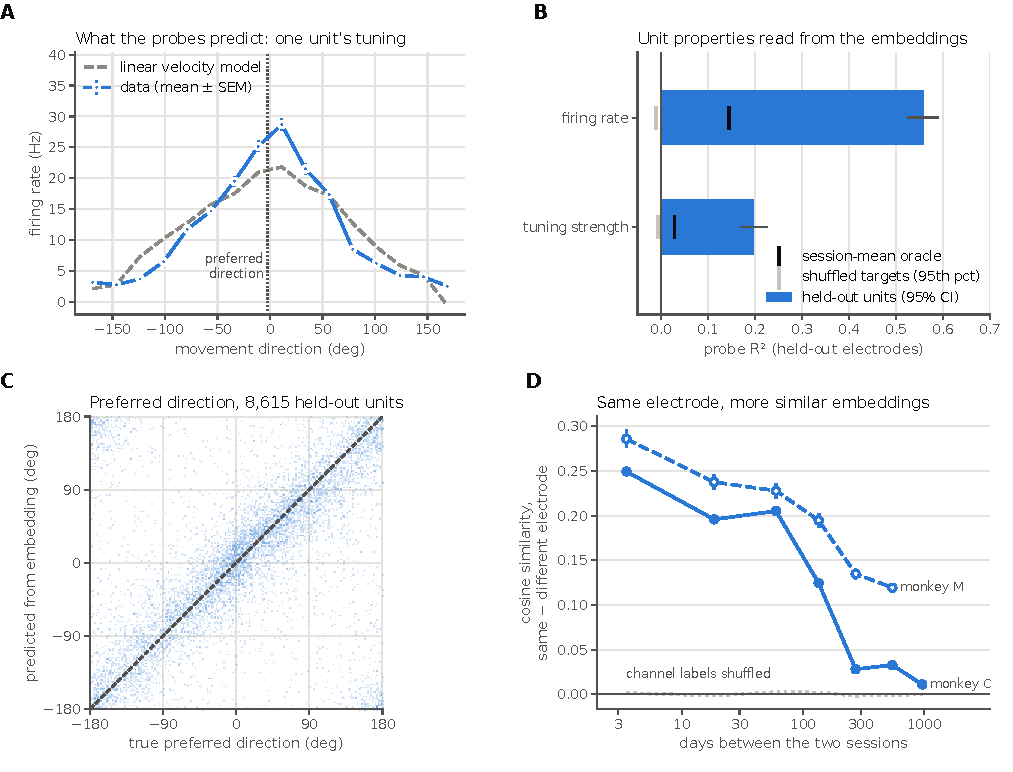
\includegraphics[width=\linewidth]{figS2_unit_embeddings}
\caption{\textbf{What the unit embeddings encode.} (A) What the probes predict: the firing rate of the
best-tuned CO unit against movement direction at its best lag, with the fitted linear velocity model
(grey, dashed); dotted: its preferred direction. (B) Held-out R$^{2}$ of linear probes from the
embeddings to firing rate and tuning strength (95\% CI over sessions); black ticks: session-mean
oracle; grey ticks: shuffled targets (95th percentile). (C) True against predicted preferred
direction for all 8,615 well-tuned held-out units. (D) Cosine similarity of same-electrode minus
different-electrode unit pairs, for pairs of sessions of monkey C (filled) and M (open) against the
days between them (mean $\pm$ SEM per bin); dotted: shuffled channel labels.}
\end{figure}

\textbf{Further results.} The rate probe is not a proxy for how often a unit fired during training: the log training spike count alone predicts log rate with R$^{2}$ 0.77, and adding the probe's prediction raises this to 0.83 (partial r 0.50). Session identity explains 2.4\% of the variance between embeddings, monkey 0.5\% and brain area 0.3\%; seven unit properties explain 8.3\% (in-sample). Units recorded on the same electrode in two different sessions have more similar embeddings (cosine) than units on different electrodes, by +0.077 (C, 2,278 session pairs), +0.175 (M, 378) and +0.267 (J, 3), and by about 0 with channel labels shuffled (p $\leq$ 0.01 for each monkey). The difference decays with the time between sessions (Spearman $-$0.72 for C, $-$0.80 for M).

\textbf{Design choices and limitations.} Properties are measured during movement, because the whole training split dilutes CO tuning about 15-fold (holds and inter-trial time), and the scored periods alone leave half of the CO units with fewer than 200 spikes. Targets are rank-transformed because tuning strength is heavily skewed. The tuning model and the probes are linear, and CO tuning is limited by the fixed set of reach directions.

\subsection{Neuron letters: how many shared codes the embeddings need}

\textbf{Question.} Each neuron has its own 128-number embedding, so the table grows with every new recording. Could neurons instead share a small set of codes (``letters''), as tokens share a vocabulary in a language model? We replace every unit embedding of a session with its code in a shared codebook and measure how much decoding survives. Nothing is trained, and no unit properties are measured: the codebooks see only the embedding table.

\textbf{Codebooks.} A codebook is fitted on the embeddings of units from \emph{other} sessions and then applied to the held-out session, so a unit never helps build its own letter. Two fitting schemes: \emph{other sessions} (5 folds of sessions, dealt within each monkey, so other days of the same monkey are in the fit) and \emph{other monkeys} (leave one monkey out). Three kinds of code, compared at equal code length in bits (log$_2$ of the number of possible codes):

\begin{itemize}
\item \emph{one alphabet}: k-means with K letters (K = 2 to 1024; K = 1 is the mean embedding);
\item \emph{parallel letters}: the embeddings are rotated onto their principal axes, the 128 axes are dealt into M blocks (M = 2, 4, 8; round-robin, so blocks carry similar variance), and each block gets its own alphabet; a unit's code is M letters;
\item \emph{coarse-to-fine letters}: a first alphabet, then further alphabets fitted to what the earlier letters missed (16 or 256 letters per stage, up to 6 stages).
\end{itemize}

Controls: \emph{area letters} (the mean embedding of the unit's brain area), \emph{random letters} (the session's k-means letters permuted among its units), and a continuous code that keeps the top d principal components (d = 1 to 64). A second run codes only each embedding's \emph{direction} (unit vector) and gives every unit back its own length; \emph{mean length} keeps each unit's own direction and gives all units the average length. Kept = R$^{2}$ $\div$ the session's own R$^{2}$. These runs use half precision (fp16) for speed; the own R$^{2}$ is computed the same way and differs from full precision by at most 5 $\times$ 10$^{-5}$.

\begin{table}[!tbp]
\centering
\small
\caption{\textbf{Share of R$^{2}$ kept when every unit embedding is replaced by its code.} Median over 99 sessions [session-bootstrap 95\% CI].}
\begin{tabularx}{\linewidth}{Ylll}
\toprule
code & bits & other sessions & other monkeys \\
\midrule
area letters & 1 & $-$0.01 & $-$0.00 \\
random letters (K = 256) & 8 & $-$0.01 & $-$0.01 \\
one alphabet, K = 16 & 4 & 0.26 [0.21, 0.30] & 0.06 [0.02, 0.10] \\
one alphabet, K = 256 & 8 & \textbf{0.86} [0.85, 0.88] & \textbf{0.09} [0.03, 0.20] \\
one alphabet, K = 1024 & 10 & 0.90 [0.89, 0.92] & 0.09 [0.03, 0.19] \\
2 parallel $\times$ 16 letters & 8 & 0.46 [0.43, 0.52] & 0.18 [0.14, 0.24] \\
coarse-to-fine, 2 $\times$ 256 & 16 & 0.93 [0.92, 0.94] & 0.28 [0.20, 0.40] \\
4 parallel $\times$ 64 letters & 24 & 0.91 [0.89, 0.92] & \textbf{0.78} [0.71, 0.82] \\
coarse-to-fine, 6 $\times$ 16 & 24 & 0.89 [0.87, 0.91] & 0.77 [0.70, 0.80] \\
coarse-to-fine, 3 $\times$ 256 & 24 & \textbf{0.95} [0.94, 0.96] & 0.47 [0.40, 0.56] \\
top 8 principal components & -- & 0.72 [0.67, 0.75] & 0.37 [0.24, 0.56] \\
top 16 principal components & -- & \textbf{0.96} [0.95, 0.97] & \textbf{0.88} [0.87, 0.91] \\
top 32 principal components & -- & 1.00 & 0.99 \\
own direction, mean length & -- & 1.00 & 1.00 \\
\bottomrule
\end{tabularx}
\end{table}

\textbf{Results.} With codebooks from other sessions, about 256 letters keep 86\% of R$^{2}$, and 1024 letters keep 90\%, not significantly more than 512 letters (0.89; Holm p = 0.93). Which letter a unit gets matters: random letters and area letters keep nothing. At equal length, one alphabet beats composed codes (8 bits: 0.86 against 0.46 for parallel and 0.56 for coarse-to-fine letters; Holm p < 10$^{-14}$); composed codes help only by going beyond about 10 bits, where three coarse-to-fine stages of 256 letters keep 95\%. Keeping the top 16 principal components keeps 96\% (slightly more than the best 24-bit code; Holm p = 0.007, though 16 exact numbers carry more information than 24 bits, so this is not a size-matched comparison) and 32 keep all of it. No small set of neuron types suffices: accuracy grows steadily with the number of letters (0.26 with 16, 0.64 with 64, 0.86 with 256) instead of saturating at a few, and the codes that work best have far more possible values than there are neurons (4 parallel letters of 64 give 16.8 million codes for 9,725 neurons). Most of the identity lies in about 16 to 32 shared directions.

With codebooks from \emph{other monkeys}, one alphabet fails (K = 256: 0.09; 0.01 for monkey C, 0.27 for J, 0.51 for M), while 24-bit composed codes still work: 4 parallel letters of 64 keep 78\% and 6 coarse-to-fine stages of 16 keep 77\%; and 16 principal components fitted on the other monkeys keep 88\%. The axes of the embedding space carry over between monkeys; the locations of whole-neuron letters do not. The failure is not the embedding's length: lengths differ by monkey (median 0.61 C, 0.79 M, 1.25 J), but replacing every unit's length by the average keeps 99.7--99.8\% of R$^{2}$ (92\% for J), and letters on direction alone fail in the same way (K = 256: 0.16 from other monkeys, against 0.83 from other sessions). Instead, monkey C's units lie in their own region of the space: for 97\% of them the nearest unit is another session of monkey C rather than a unit of M or J (39\% for M, 28\% for J).

\begin{figure}[!tbp]
\centering
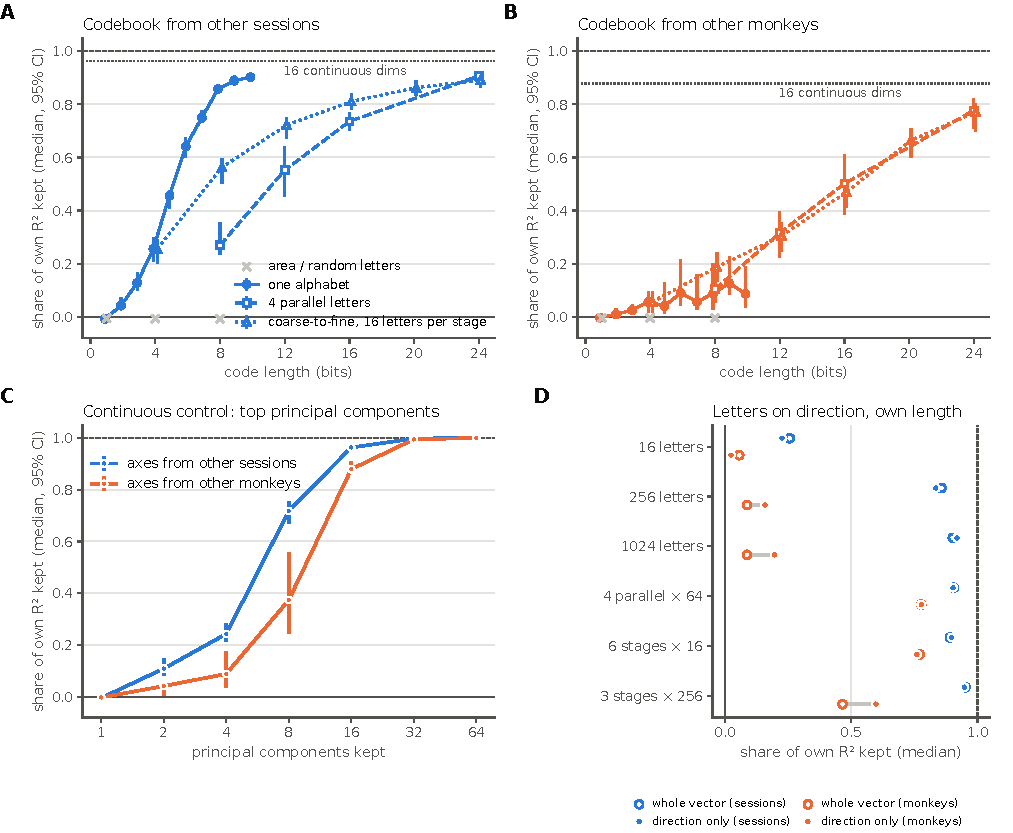
\includegraphics[width=\linewidth]{figS3_neuron_letters}
\caption{\textbf{Neuron letters.} (A) Share of R$^{2}$ kept against code length when every unit embedding of
a session is replaced by its code in a codebook fitted on other sessions (median over 99 sessions,
95\% CI): one alphabet (k-means), 4 parallel letters (one alphabet per block of principal axes) and
coarse-to-fine letters (16 letters per stage); crosses: area and random letters; dotted: 16
principal components. (B) As A, with codebooks fitted on the other monkeys. (C) The continuous
control: top principal components, with axes from other sessions (blue) or other monkeys (orange).
(D) Letters fitted on the direction of each embedding, with each unit keeping its own length
(filled), against letters on the whole vector (open).}
\end{figure}

\textbf{Further results.} Letters fitted on all units (for description only) track recording conditions weakly: adjusted mutual information of a 256-letter code with session 0.07, brain area 0.06, monkey 0.05 and task 0.03. Units on the same electrode in two different sessions share a 256-letter code 7.8\% of the time, against 0.8\% for units on different electrodes of the same monkey (242,712 same-electrode pairs).

\textbf{Design choices and limitations.} k-means uses Euclidean distance, three restarts and one seed; fits are reproducible to about 10$^{-16}$ (multithreading). When monkey C is held out, the codebook is fitted on only 2,682 units of M and J, against 7,043 of C, so the cross-monkey result is partly a test of how well a small population covers a large one. The codebooks are fitted to the embeddings POYO-MP learned, not trained into the model; a model trained with shared codes could organise its embeddings differently. Codes are assigned from each unit's own embedding, so this tests how much a shared code can hold, not how to find a new neuron's code from its activity. We did not test directly whether the embeddings form separate clusters; the conclusion that they are not a small set of types rests on how accuracy grows with the number of letters.

\setcounter{table}{0}
\renewcommand{\thetable}{C\arabic{table}}
\section{Tests of the network}

\subsection{Missing neurons}

\textbf{Lesions.} Each test window is lesioned before tokenization. Under \emph{remove}, a unit is deleted from the session's unit list, so it gets no [START]/[END] tokens, and the remaining units are re-indexed as \texttt{UnitDropout} does in training; under \emph{silence}, only its spikes are deleted. Each seed fixes one random order of units per session, so the same units are lost in every window and for both lesion types, and lesioned sets are nested across conditions (3 seeds, 3,528 evaluations).

\textbf{Did training see it?} Simulating \texttt{UnitDropout} with the library's own sampler (20,000 draws per session), a condition is \emph{in training} for a session if at least 1\% of its training windows kept that many units or fewer.

\textbf{Refitted ridge.} The ridge decoder of Appendix C.2 (100 ms bins, 300 ms of history), refitted from scratch on the kept units of every lesion.

\begin{table}[!tbp]
\centering
\scriptsize
\setlength{\tabcolsep}{4pt}
\caption{\textbf{Removing vs silencing lost units.} Per-session $\Delta$R$^{2}$ (mean of 3 seeds), mean over sessions; paired Wilcoxon test of remove $-$ silence, Holm-corrected over conditions. ``Keep n'' conditions include only sessions with more than n units.}
\begin{tabular}{llllllll}
\toprule
condition & sessions & in training & $\Delta$R$^{2}$ remove & $\Delta$R$^{2}$ silence & \begin{tabular}[b]{@{}l@{}}remove $-$ \\ silence\end{tabular} & remove better & Holm p \\
\midrule
10\% lost & 99 & 95\% & $-$0.011 & $-$0.011 & +0.001 & 64\% & 0.031 \\
25\% lost & 99 & 87\% & $-$0.031 & $-$0.038 & +0.008 & 89\% & < 0.001 \\
50\% lost & 99 & 46\% & $-$0.094 & $-$0.160 & +0.066 & 99\% & < 0.001 \\
75\% lost & 99 & 20\% & $-$0.311 & $-$0.566 & +0.254 & 99\% & < 0.001 \\
keep 30 & 95 & 0\% & $-$0.123 & $-$0.337 & +0.214 & 97\% & < 0.001 \\
keep 20 & 97 & 0\% & $-$0.237 & $-$0.530 & +0.293 & 99\% & < 0.001 \\
\bottomrule
\end{tabular}
\end{table}

\begin{figure}[!tbp]
\centering
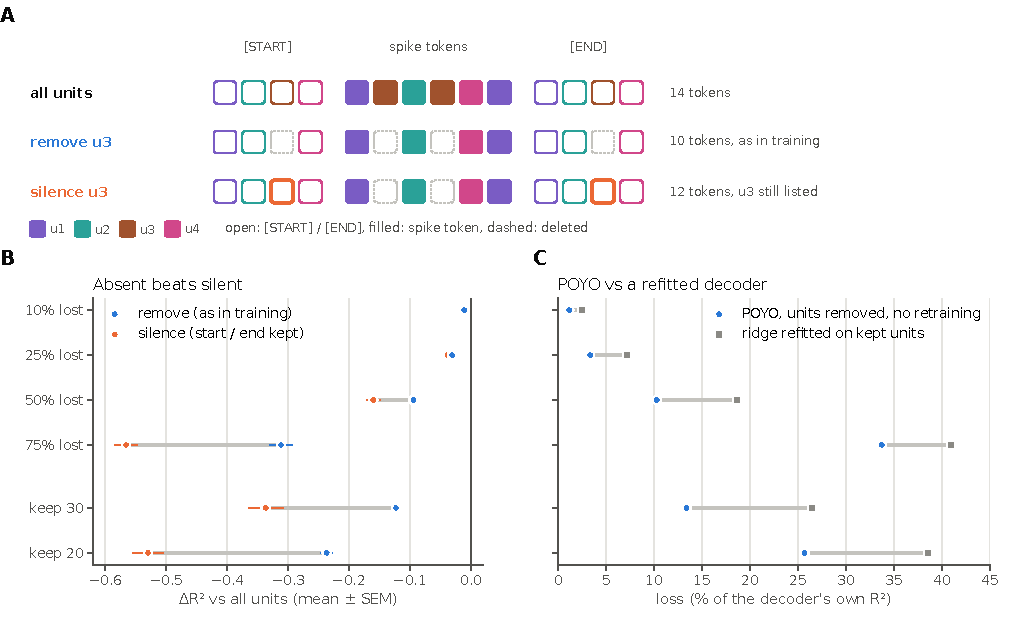
\includegraphics[width=\linewidth]{figS4_missing_neurons}
\caption{\textbf{Missing neurons.} (A) Tokens of a window with four units (one colour per unit; open:
[START]/[END], filled: spike tokens, dashed: deleted). Removing unit u3 deletes its spike tokens and
its [START]/[END] tokens; silencing it deletes only its spike tokens, so the model still sees the
unit listed (orange outline). (B)
$\Delta$R$^{2}$ relative to all units when units are removed (blue) or silenced (orange) (mean $\pm$ SEM across
sessions, 3 seeds averaged). (C) Loss as a percentage of each decoder's own all-unit R$^{2}$ for POYO-MP
with the units removed and no retraining (blue) and for a ridge decoder refitted on the kept units
(grey).}
\end{figure}

\textbf{Further results.} Removal roughly halves the damage of silencing at large losses (45--55\% less at 75\% lost or 20 units kept), including in conditions that training never produced (keep 30 and keep 20). Relative to its own R$^{2}$, POYO without retraining loses less than the refitted ridge: 1.2\% vs 2.5\% (10\% lost), 3.4\% vs 7.2\% (25\%), 10.3\% vs 18.7\% (50\%) and 33.7\% vs 41.0\% (75\%); every difference has Holm p < 0.001.

\subsection{Spike timing}

\textbf{Perturbations.} Each test window is perturbed after slicing and before tokenization, keeping every unit's spike count. \emph{Snap} moves each spike to the centre of its bin; \emph{bin shuffle} moves it to a uniform random time within its bin, drawn from a hash of (seed, unit, spike time), so that a spike moves to the same time in every window that contains its bin; \emph{window shuffle} moves it to a random time within its 1 s window. Bins (1, 2, 5, 10, 20, 50, 75, 100, 150, 200, 333 and 500 ms) lie on a grid anchored to absolute recording time; a bin cut by a window edge is clipped to the window, so spikes never leave it. [START]/[END] tokens are unaffected, and a zero-size perturbation reproduces the baseline bit for bit (79 tests cover these properties). Bin and window shuffle use 3 seeds.

\textbf{Binned ridge control.} Ridge regression on spike counts per unit, for each session and bin size (10--500 ms), with $\lceil$250 ms / bin$\rceil$ bins of history, trained on the training split with POYO's loss weights, the penalty chosen on the validation split, and scored on the same test points as POYO.

\begin{table}[!tbp]
\centering
\small
\setlength{\tabcolsep}{4pt}
\caption{\textbf{Change in R$^{2}$ when spike times are moved.} Mean $\pm$ SEM across sessions (78 CO, 21 RT). At 10 ms, some effects are statistically detectable (bin shuffle on CO, p = 0.0005); from 20 ms on, every setting is (Holm p $\leq$ 0.003).}
\begin{tabular}{lllll}
\toprule
\begin{tabular}[b]{@{}l@{}}$\Delta$R$^{2}$ (mean $\pm$ \\ SEM)\end{tabular} & CO bin shuffle & RT bin shuffle & CO snap & RT snap \\
\midrule
1 ms & $-$0.0000 $\pm$ 0.0000 & $-$0.0000 $\pm$ 0.0000 & $-$0.0001 $\pm$ 0.0000 & $-$0.0004 $\pm$ 0.0001 \\
\textbf{10 ms} & \textbf{$-$0.0002 $\pm$ 0.0001} & \textbf{$-$0.0002 $\pm$ 0.0001} & \textbf{$-$0.0002 $\pm$ 0.0001} & \textbf{$-$0.0006 $\pm$ 0.0002} \\
20 ms & $-$0.0007 $\pm$ 0.0001 & $-$0.0009 $\pm$ 0.0002 & $-$0.0004 $\pm$ 0.0001 & $-$0.0010 $\pm$ 0.0002 \\
50 ms & $-$0.0029 $\pm$ 0.0003 & $-$0.0048 $\pm$ 0.0006 & $-$0.0012 $\pm$ 0.0002 & $-$0.0026 $\pm$ 0.0004 \\
100 ms & $-$0.0128 $\pm$ 0.0007 & $-$0.0203 $\pm$ 0.0022 & $-$0.0050 $\pm$ 0.0004 & $-$0.0095 $\pm$ 0.0011 \\
200 ms & $-$0.0628 $\pm$ 0.0027 & $-$0.0897 $\pm$ 0.0069 & $-$0.0525 $\pm$ 0.0021 & $-$0.0695 $\pm$ 0.0051 \\
500 ms & $-$0.337 $\pm$ 0.012 & $-$0.376 $\pm$ 0.017 & $-$0.656 $\pm$ 0.018 & $-$0.717 $\pm$ 0.023 \\
window shuffle & $-$0.874 $\pm$ 0.010 & $-$0.784 $\pm$ 0.014 &  &  \\
\bottomrule
\end{tabular}
\end{table}

\begin{figure}[!tbp]
\centering
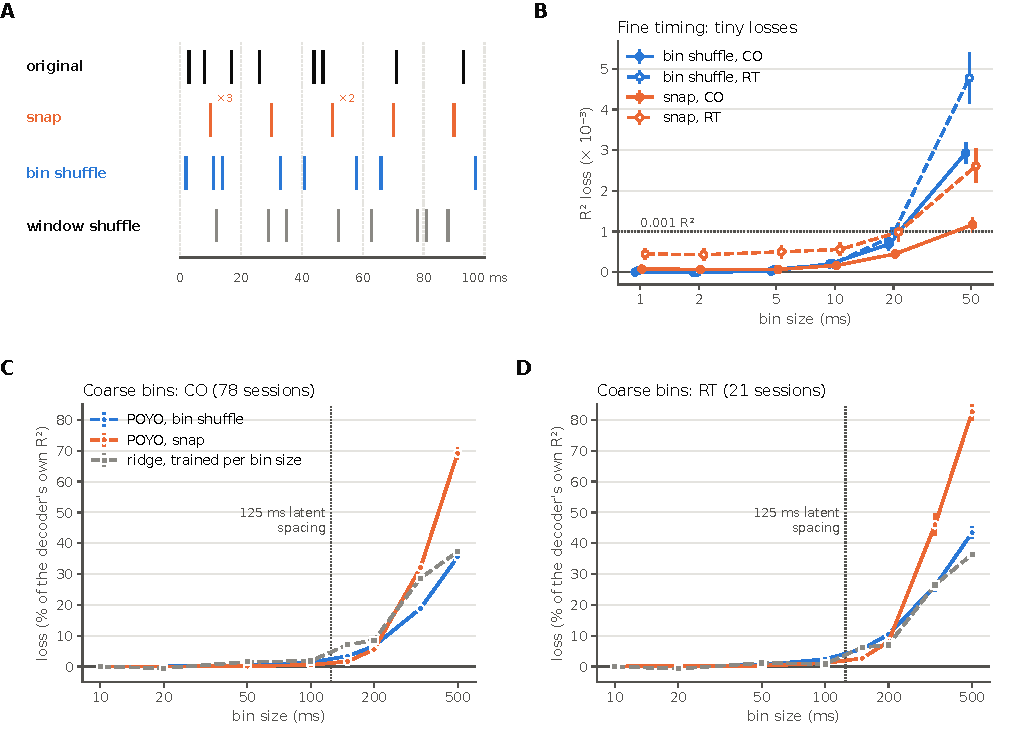
\includegraphics[width=\linewidth]{figS5_spike_timing}
\caption{\textbf{Spike timing.} (A) The timing perturbations, shown for 20 ms bins: snap (orange) moves
each spike to the centre of its bin, bin shuffle (blue) to a random time within it, and window
shuffle (grey) to a random time within the 1 s window; spike counts never change. (B) R$^{2}$ loss for
bins of 1--50 ms (mean $\pm$ SEM across sessions; filled, solid: CO, 78 sessions; open, dashed: RT, 21
sessions); dotted: a loss of 0.001 R$^{2}$. (C, D) Loss as a percentage of each decoder's own R$^{2}$ for bins
of 10--500 ms, for POYO-MP under bin shuffle and snap and for a ridge decoder trained at each bin
size (grey, dashed), on CO (C) and RT (D). Dotted: POYO-MP's 125 ms latent spacing.}
\end{figure}

\textbf{Further results.} On RT, snap costs a small constant 0.0004--0.0006 R$^{2}$ even at 1--10 ms, where bin shuffle costs nothing: an effect of the regular grid, not of lost timing. Under bin shuffle, RT is about 1.4--1.7 times more sensitive than CO at 50--200 ms.

\textbf{Design choices and limitations.} Window shuffle draws each window independently, and overlapping predictions are averaged, so it is not one coherent shuffled recording. The ridge's history varies with bin size (250--500 ms). Behaviours with faster dynamics, or other brain areas, could depend more on fine timing.

\end{document}
